\documentclass[10pt,a4paper,twoside,openright,titlepage,twocolumn]{article}
\usepackage[utf8]{inputenc}
\usepackage[T1]{fontenc}
\usepackage{amsmath}
\usepackage{amssymb}
\usepackage{graphicx}
\usepackage{xcolor}
\usepackage{wrapfig}
\usepackage{siunitx}
\usepackage{titlesec}
\usepackage{titlepic}
\usepackage[export]{adjustbox}
\usepackage[left=6.00mm, right=6.00mm, top=6.00mm, bottom=12.00mm]{geometry}
\usepackage{listings}



\graphicspath{ {./Images/} }

\definecolor{formulablue}{RGB}{219,219,255}
\newcommand{\formula}[1]{\colorbox{formulablue}{#1}}

\newcommand{\unitText}[3]{\noindent\textit{#1} : #2 [#3]}

\definecolor{refrot}{RGB}{183,28,42}
\definecolor{LightGray}{gray}{0.9}
\definecolor{ForestGreen}{RGB}{34,139,34}
\newcommand{\refskript}[1]{\textcolor{refrot}{#1}}
\newcommand{\refskriptP}[1]{\textcolor{refrot}{Skript S.#1}}

% Define the Gruvbox light colors
\definecolor{gruvbox_bg}{HTML}{fbf1c7}
\definecolor{gruvbox_fg}{HTML}{3c3836}
\definecolor{gruvbox_yellow}{HTML}{d79921}
\definecolor{gruvbox_red}{HTML}{cc241d}
\definecolor{gruvbox_green}{HTML}{98971a}
\definecolor{gruvbox_blue}{HTML}{458588}
\definecolor{gruvbox_purple}{HTML}{b16286}
\definecolor{gruvbox_aqua}{HTML}{689d6a}
\definecolor{gruvbox_orange}{HTML}{d65d0e}

% Setup Source Code
\lstset{ 
	backgroundcolor=\color{white},   % choose the background color; you must add \usepackage{color} or \usepackage{xcolor}; should come as last argument
	basicstyle=\ttfamily\footnotesize,   % the size of the fonts that are used for the code
	breakatwhitespace=true,         % sets if automatic breaks should only happen at whitespace
	breaklines=true,                 % sets automatic line breaking
	captionpos=b,                    % sets the caption-position to bottom
	commentstyle=\color{gruvbox_aqua},    % comment style
	emph={int, double, string, cout},
	emphstyle=\color{gruvbox_red},
	escapeinside={\%*}{*)},          % if you want to add LaTeX within your code
	extendedchars=true,              % lets you use non-ASCII characters; for 8-bits encodings only, does not work with UTF-8
	frame=single,	                   % adds a frame around the code
	identifierstyle=\color{gruvbox_fg},
	keepspaces=true,                 % keeps spaces in text, useful for keeping indentation of code (possibly needs columns=flexible)
	keywordstyle=\color{gruvbox_orange},
	language=C,                      % the language of the code
	numbers=left,
	numberstyle=\tiny,
	numbersep=5pt,                   % how far the line-numbers are from the code
	rulecolor=\color{gruvbox_fg},    % if not set, the frame-color may be changed on line-breaks within not-black text (e.g. comments (green here))
	showspaces=false,                % show spaces everywhere adding particular underscores; it overrides 'showstringspaces'
	showstringspaces=false,          % underline spaces within strings only
	showtabs=false,                  % show tabs within strings adding particular underscores
	stepnumber=2,                    % the step between two line-numbers. If it's 1, each line will be numbered
	stringstyle=\color{gruvbox_green},
	tabsize=4,	                   % sets default tabsize to 2 spaces
	title=\lstname,                   % show the filename of files included with \lstinputlisting; also try caption instead of title
	literate={~} {$\sim$}{1},
	xleftmargin=\parindent,
	xrightmargin=\parindent
}


\setlength{\parindent}{0pt}

\titlespacing*{\section}{0pt}{12pt}{0pt}
\titlespacing*{\subsection}{0pt}{0pt}{0pt}
\titlespacing*{\subsubsection}{0pt}{0pt}{0pt}

\title{\vspace{50mm}SigSys2 \\ [1ex] \large Formelsammlung}
\author{Sebastian Humbel}
\titlepic{\vspace{50mm}
\includegraphics[width=0.25\textwidth]{Elvis}}




\begin{document}
	\maketitle
	%\section{Section1}
\subsection{Subsection1}
\begin{minipage}[t]{0.3\textwidth}
	\vspace{0pt}								% Abbildung hier einfügen
	\includegraphics[width=\textwidth]{"Bild"}
\end{minipage}\hspace{0.05\textwidth}
\begin{minipage}[t]{0.65\textwidth}
	\vspace{0pt}								% Beschreibung und Formeln hier einfügen
	Beschreibung zum Thema. \refskript{10}\\
	\formula{$1+1 = 2$}
	\formula{$1+1 = 2$}
\end{minipage}
\vspace{2mm}

\noindent
\begin{minipage}{0.5\textwidth}
	\unitText{Symbol}{Beschreibung}{$Einheit$}
\end{minipage}%%%
\begin{minipage}{0.5\textwidth}
	\unitText{Symbol}{Beschreibung}{$Einheit$}
\end{minipage}




\section{Section2}
\subsection{Subsection2}
\begin{minipage}[t]{0.3\textwidth}
	\vspace{0pt}								% Abbildung hier einfügen
	\includegraphics[width=\textwidth]{"Bild"}
\end{minipage}\hspace{0.05\textwidth}
\begin{minipage}[t]{0.3\textwidth}
	\vspace{0pt}								% Beschreibung und Formel hier einfügen
	Beschreibung zum Thema und ein Test wie breit
	man schreiben kann. \refskript{10}\\
	\begin{center}
		\formula{$1+1 = 2$}\\
		\formula{$\sum{3a+x}$}
	\end{center}
\end{minipage}\hspace{0.05\textwidth}
\begin{minipage}[t]{0.3\textwidth}
	\vspace{0pt}								% Einheiten hier einfügen
	\unitText{Symbol}{Beschreibung}{$Einheit$}
\end{minipage}




	\section{GPIO \refskript{8.1, 8.2}}


	\section{Interrupt Concepts \refskript{7.1, 7.2}}
A Interrupt is a signal indicating the occurrence of an event that needs immediate CPU attention.
There exist different types of Interrupts:
\begin{itemize}
	\itemsep-.5em 
	\item Hardware triggers
	\item Software triggers
	\item CPU exceptions
\end{itemize}

\begin{lstlisting}[language=c]
PxDIR &= ~0x01;	// Set Px.0 as input
PxDIR |=  0x02;	// Set Px.1 as output
PxOUT &= ~0x02;	// Clear LED on Px.1
PxIE  |=  0x01;	// IRQ when SW1 is pressed
...
__interrupt void portx_ISR(void) {
	PxOUT ^=  0x02;
}
\end{lstlisting}\vspace{-25px}

\subsection{Maskabe vs. Nonmaskable \refskript{7.1.2}}
\textit{Maksable}: Can be blocked (masked), trough flags. Most common type of interrupt. Disabled upon RESET.

\textit{Non-maskable} interrupts (NMI): Cannot be masked, thus are always served. Reserved for system critical events

Also see \refskript{7.2.2} and \refskript{7.2.3}


\subsubsection{Interrupt Flow}
\includegraphics[width=.6\columnwidth, center]{"InterruptFlow"}

Interrupt kann über intrinsische Funktionen eingestellt werden.
Alternativ mit enable\_interrupt() funktion.


\subsubsection{Interrupt Service Sequence \refskript{7.1.3}}
PC speicher den aktuellen ort im code bevor der Interrupt ausgeführ wird.
SR wird auf dem stack gespeichert

\subsubsection{Interrupt Identification Methods \refskript{7.1.4}}
\textit{Non-vectored systems (1)} don't know, what triggered the interrupt and have to identify the interrupt source within the ISR.

\textit{Vectored interrupts (2)} Have an ID for each interrupt type an can jump directly to the desired ISR.

\textit{Auto-vectored interrupts (3)} have predefined addresses / fix vectors for the different interrupts.

\subsubsection{Interrupt Priority Handling \refskript{7.1.5}}
(1) \textit{Polling order of SRQ flags} decides priority (if else if define the interrupt priority)

(2) \textit{Daisy Chain-based Arbitration} defines the priority through hardwired logic. Used by the MSP430.

(3) \textit{Interrupt controller-based Arbitration} allows priority configuration by the user.

\subsection{Interrupt Software Design \refskript{7.3}}
\begin{lstlisting}[language=c]
// main.c
int main(void){
	hal_gpio_init();
	hal_gpio_interruptCallbackFctRegister(
					GPIO_S1,_s1_callbackFct);
}

static void _s1_callbackFct(void){
	...
}
\end{lstlisting}\vspace{-25px}
\begin{lstlisting}[language=c]
// hal_gpio.h
void hal_gpio_init(void);
void hal_gpio_interruptCallbackFctRegister(
			gpioPeripherie_t gpio, pFctHandler pCallbackFct);
\end{lstlisting}\vspace{-25px}
\begin{lstlisting}[language=c]
// hal_gpio.c
void hal_gpio_init(void) { // ... }
void hal_gpio_interruptCallbackFctRegister(
		gpioPeripherie_t gpio, pFctHandler pCallbackFct) {
			_hal_gpio_callbackFct[0] = pCallbackFct;
}

#pragma vector=PORT1_VECTOR
__interrupt void _port1_ISR(void) {
	// ...
	_hal_gpio_callbackFct[0](); // call back application code
}
\end{lstlisting}\vspace{-25px}




	\section{Clock System}
\subsection{Clock Sources \refskript{6.3}}
Clock settings in \textit{CSCTL} register.\\
Voltage Swing $V_{SW} = V_{OH} - V_{OL}$ : Amplitude from low to high.\\
Frequency $f_{clk} = \dfrac{1}{T_{clk}}$ : Number of cycles per second\\
Duty Cycle $DC = \dfrac{t_{high}}{T_{clk}} * 100 \%$ : Ratio of high time to period\\
Edge Speed $t$ and $t_f$ : Rising and falling times

\includegraphics[width=\columnwidth]{"clock"}

\subsection{Clock Stability \refskript{6.3.1}}
Statistical measure of the maximum allowable parameter fluctuations of a clock signal
over a given time interval.

\begin{minipage}[t]{0.5\columnwidth}
	Possible factors:
	\begin{itemize}
		\itemsep-.5em 
		\item type of oscillator
		\item capacitive load
		\item ageing
		\item supply voltage or temperature
	\end{itemize}
\end{minipage}
\begin{minipage}[t]{0.5\columnwidth}
	Short- and long-term effects:
	\begin{itemize}
		\itemsep-.5em 
		\item Clock Jitter
		\item Clock Drift
	\end{itemize}
\end{minipage}
\vspace{2mm}

\subsection{Source Selection \refskript{6.3.2}}
Choose the lowest frequency that allows for a reliable and correct system operation.
Adjust the frequency to the speed of the fastest event.


\subsection{Internal vs. External Clock \refskript{6.3.3}}

\begin{minipage}[t]{0.5\columnwidth}
	\textbf{Internal}
	
	Pro:
	\begin{itemize}
		\itemsep-.5em 
		\item Reduce external component count
		\item Less expensive
		\item Induce lower power consumption
	\end{itemize}
	Con:
	\begin{itemize}
		\itemsep-.5em 
		\item Reduced clock stability
		\item Less flexibility
		\item Narrower bandwidth
	\end{itemize}
\end{minipage}
\begin{minipage}[t]{0.5\columnwidth}
	\textbf{External}
	
	Pro:
	\begin{itemize}
		\itemsep-.5em 
		\item Wider choice of frequencies
		\item More design flexibility
	\end{itemize}
	Con:
	\begin{itemize}
		\itemsep-.5em 
		\item Increment the external component count
		\item Higher clock speeds induce higher power
		consumption
	\end{itemize}
\end{minipage}
\vspace{2mm}

\subsection{RC-based Oscillator}
\includegraphics[width=0.7\columnwidth, center]{"rcbased_oscillator"}

\subsection{Quartz Crystal Oscillators \refskript{6.3.4}}
Based on mechanical resonance of a vibrating piezoelectric crystal.

\subsection{Pierce Crystal Oscillator \refskript{6.3.4}}
Series Resonant Oscillator

\subsection{Colpitts Crystal Oscillator \refskript{6.3.4}}
Parallel Resonant Oscillator

\subsection{Oscillator Startup Time \refskript{6.3.4}}

\section{The MSP430 System Clock \refskript{6.4}}
\includegraphics[width=0.7\columnwidth, center]{"MSP430clocksystem"}

\subsection{DCO Clock}
Digitally controlled oscillator
\begin{enumerate}
	\itemsep-.5em 
	\item Select a frequency range (DCORSEL)
	\item Select the frequency within that range (DCO)
	\item Setup Modulation (MOD)
\end{enumerate}
\includegraphics[width=0.5\columnwidth]{"DCOwide"}
\includegraphics[width=0.5\columnwidth]{"DCOnarrow"}

\includegraphics[width=0.5\columnwidth]{"DCOmod1"}
\includegraphics[width=0.5\columnwidth]{"DCOmod2"}









	\section{Timer \& Event Counters \refskript{7.4}}
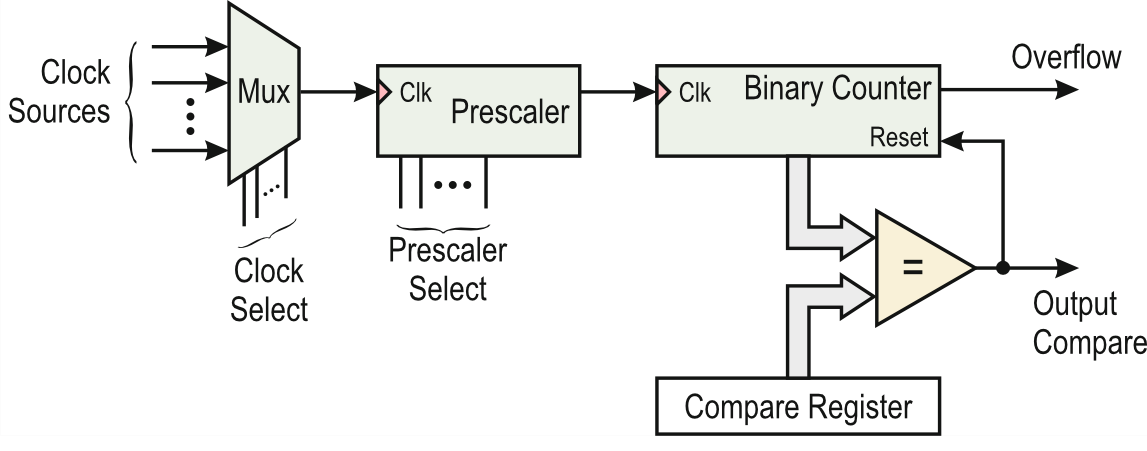
\includegraphics[width=\columnwidth]{"Images/TimerFuntionsweise.png"}

\subsection{Signature Timer Applications \refskript{7.4.3}}
\textit{Watchdog timer} is secured through a password in the \textit{WDTCTL} register.
\textit{Real-Time Clocks} provides absolute time (second, minute, hour, day, month, week).
\textit{Baud Rate Generation} can provide clock base for baud rate.

\begin{minipage}{.5\columnwidth}
	\formula{$\mathit{baudrate} = \dfrac{f_{\mathit{clk}}}{\mathit{PS} \cdot \mathit{TopCount}}$}
\end{minipage}
\begin{minipage}{.5\columnwidth}
	\unitText{$\mathit{PS}$}{Prescale Factor}{1}\\
	\unitText{$f_{\mathit{clk}}$}{Clock frequency}{Hz}\\
	\unitText{$\mathit{TopCount}$}{Compare value}{1}
\end{minipage}

\subsubsection{MSP430 Timer Support \refskript{7.4.4}}

Operating Modes

Input Capture Operation

Measuring a Signal Width

Output Compare Operation
	\section{Low-Power Modes \refskript{7.3.6}}
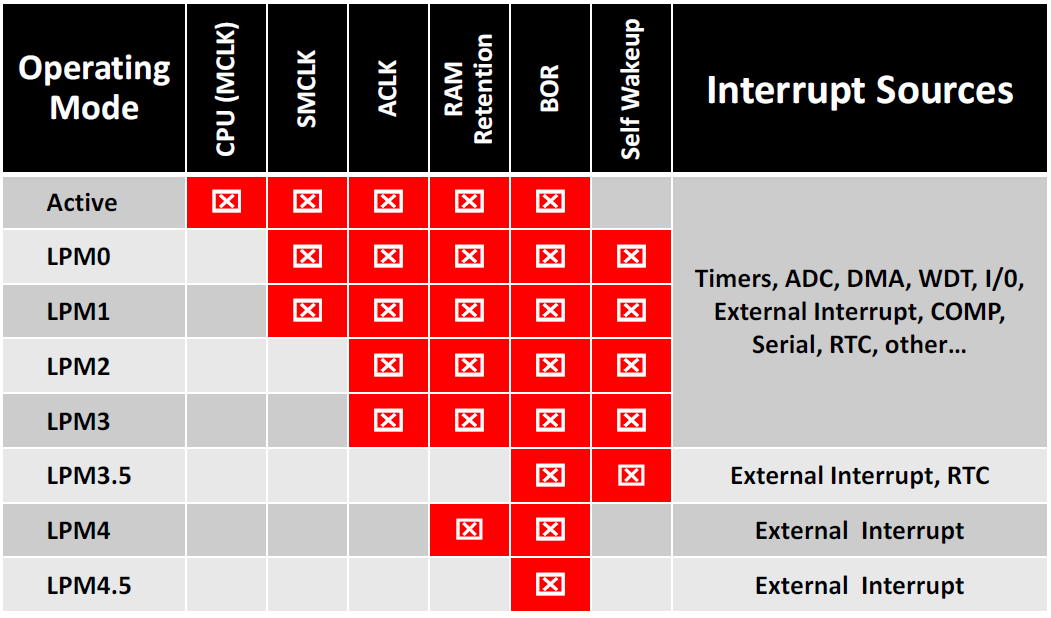
\includegraphics[width=.8\columnwidth, center]{Images/LPO_interrupts.png}

\subsection{Activity Profiles}

\subsection{Power Consumption in CMOS Technology}
\begin{minipage}{0.5\columnwidth}
	\vspace{0pt}
	\formula{$P \sim \alpha C_L V_{dd}^2 f$}
	\formula{$E \sim  \alpha C_L V_{dd}^2 f t$}
	\formula{$E \sim \alpha C_L V_{dd}^2 \mathit{(\# cycles)}$}
	
	\formula{$\tau \sim C_L \dfrac{V_dd}{(V_dd - V_T)^2}$}
	\formula{$f \sim \dfrac{1}{\tau} \sim V_{dd}$}
\end{minipage}
\begin{minipage}{0.5\columnwidth}
	\vspace{0pt}
	\unitText{$V_{dd}$}{supply voltage}{\unit{V}}\\
	\unitText{$V_T$}{threshold voltage}{\unit{V}}
	\unitText{$\alpha$}{switching activity}{\unit{1}}\\
	\unitText{$C_L$}{load capacity}{\unit{F}}\\
	\unitText{$f$}{clock frequency}{\unit{Hz}}\\
	\unitText{$\tau$}{Gate delay}{\unit{ms}}
\end{minipage}
\vspace{2mm}


\subsection{Interrupts and Low-Power Modes}
Low power modes are configured with the bits \textit{CPUOFF}, \textit{OSCOFF}, \textit{SCG0} and \textit{SCG1} in the \textbf{Status Register} (SR, also called R2).

\subsection{CCS6 Intrinsic Functions for MSP430}
\begin{lstlisting}[language=c]
	#include <intrinsics.h>
\end{lstlisting}

\subsection{Low-Power Optimization}
Replace software with hardware peripherals.
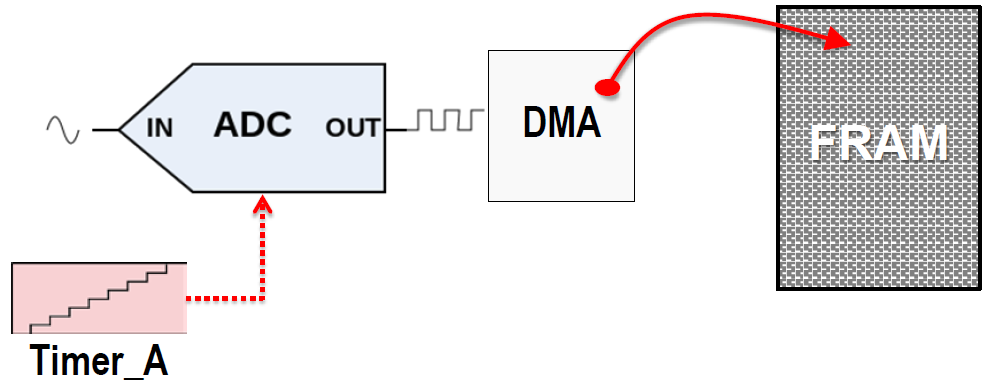
\includegraphics[width=0.8\columnwidth, center]{Images/LPM_replace_hw_with_sw.png}

\section{Real-Time Clock (RTC) \refskript{7.4.3}}
\subsection{RTC Interrupts}
\begin{enumerate}
	\itemsep-.5em 
	\item Alarm
	\item Interval Timer
	\item Prescaler 0
	\item Prescaler 1
	\item Ready for Register operation
\end{enumerate}

Example 1: Time Event
\begin{lstlisting}[language=C]
int main (void)
{
	WDTCTL = WDTPW | WDTHOLD;	//stop watchdog
	//disable high-impedance ports
	PM5CTL0 &= ~LOCKLPM5;
	//just for testing (P1.0 / LED1)
	P1DIR |= 0x01;
	P1OUT &= ~0x01;
	
	PJSEL0 = BIT4 | BIT5; //Init. LFXT pins
		
	//Configure LFXT 32kHz crystal
	CSCTL0_H = CSKEY >> 8;	//Unlock CS reg.
	CSCTL4 &= ~LFXTOFF;			//Enable LFXT
	do
	{
		//Clear LFXT fault flag
		CSCTL5 &= ~LFXTOFFG;
		SFRIFG1 &= ~OFIFG;
		//Test oscillator fault flag
	} while (SFRIFG1 & OFIFG);
	CSCTL0_H = 0;	//Lock CS registers
		
	//write RTCKEY to unlock RTC reg. for write
	RTCCTL0_H = 0xA5;
	//hold RTC, clock from output of RT1PS,
	// RTCTEVIFG on 8-bit overflow
	RTCCTL1 = 0x48;
		
	//Enable time event interrupt
	RTCCTL0_L = 0x40;
	//prescale timer 0: divided by 64
	RTCPS0CTL = 0x2800;
	//prescale timer 1: out from RT0PS, div. by 2
	RTCPS1CTL = 0x8000;
	//Enable RTC
	RTCCTL1 &= ~0x40;
	//Enter LPM3 with interrupt enabled
	__bis_SR_register(LPM3_bits + GIE);
		
	while (1)
	{}
}
\end{lstlisting}

Example 2: RTC Calendar
\begin{lstlisting}[language=C]
//BCD, hold RTC, RTCMode, one minute overflow
RTCCTL1 = 0xE0;

RTCSEC = 0x00;	//Set Seconds
RTCMIN = 0x00;	//Set Minutes
RTCHOUR = 0x10;	//Set Hours
RTCDOW = 0x03;	//Set DOW (sunday = 0)
RTCDAY = 0x18;	//Set Day
RTCMON = 0x10;	//Set Month
RTCYEAR = 0x2023;	//Set Year

//setup alarm
//enable minutes alarm, minutes = 1 and others are don't care
// --> so an alarm is generated on 00:01:00, 01:01:00, ...
RTCAMIN = 0x81;
RTCAHOUR = 0x00;
RTCADOW = 0x00;
RTCADAY = 0x01;

RTCCTL0_L = 0x60;
//Enable time event & alarm interrupt
RTCCTL1 &= ~0x40;
//Enable RTC
__bis_SR_register(LPM3_bits + GIE); //Enter LPM3 w/ interrupt
while (1)
{}
\end{lstlisting}





	\section{Serial Communication \refskript{9.1}}

\begin{itemize}
	\itemsep-.5em 
	\item \textbf{Parallel} n bits are transferred simultaneously in parallel
	\item \textbf{Serial} n bits are transferred serially, i.e., one after the other \\ Minimal duration of transfer: $n \cdot t_{Bit}$
\end{itemize}

\subsection{Types of Serial Channels \refskript{9.2}}
\begin{itemize}
	\itemsep-.5em 
	\item Simplex
	\item Half duplex
	\item Full duplex
\end{itemize}

\subsubsection{Serial Channel Topologies}

\subsection{Asynchronous Serial Communication \refskript{9.3}}
Asynchronous Packet Format \refskript{9.3.1}
\begin{itemize}
	\itemsep-.5em 
	\item \textbf{Header} 1 Start bit
	\item \textbf{Body} 5 to 8 bits character \\ optional 1 parity bit
	\item \textbf{Footer} 1/1.5/2 Stop bits
\end{itemize}
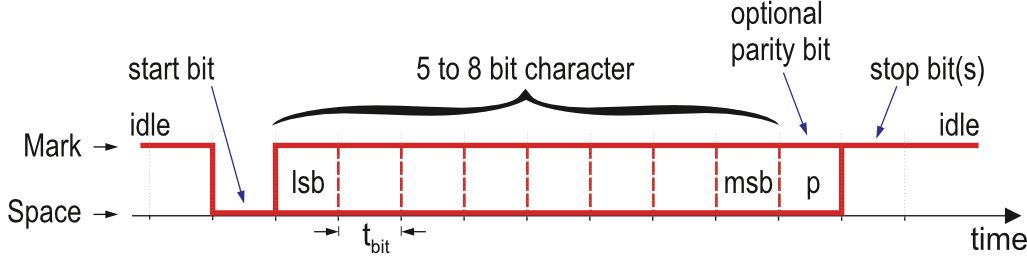
\includegraphics[width=\columnwidth]{"Images/async_package_format.png"}

Bit-Sampling at Receiver-Side: Too Slow
\formula{$\dfrac{\Delta t_\mathit{max}}{1 \mathit{Bit}} = \pm \dfrac{t_{Bit}}{2 \cdot \mathit{Framelänge}}  = \pm \dfrac{1 \mathit{Bit}}{2 \cdot \mathit{Baudrate} \cdot \mathit{Framelänge}}$}









	\subsubsection{UART \refskript{9.3.4}}
\begin{itemize}
	\itemsep-.5em
	\item Handshaking Lines \refskript{9.3.6}
	\begin{itemize}
		\itemsep-.5em 
		\item \textbf{DSR} Data Set Ready
		\item \textbf{DTR} Data Terminal Ready
		\item \textbf{RTS} Request to Send
		\item \textbf{CTS} Clear to Send
	\end{itemize}
	\item Communication Lines
	\begin{itemize}
		\itemsep-.5em
		\item \textbf{TxD} Transmitted Data
		\item \textbf{RxD} Received Data
	\end{itemize}
\end{itemize}

UART configuration \refskript{9.3.7}


\subsubsection{Baud rate}
Bit rate: Bits per second\\
Baud rate: Symbols per second

\subsubsection{RS-232 \refskript{9.3.8}}
Point to point connection.
The transfer-speed is highly dependent on the transmission line length.

\subsubsection{RS-422}
Bus connection with a maximum of 10 receivers (more with repeaters or buffers).

\subsubsection{RS-485}
Improved characteristics over RS-422 with up to 32 drivers and 32 receivers.

\subsection{Ring Buffer}
A ring buffers works with the FIFO principle.

\begin{lstlisting}[language=C]
// --- Defines
#define _UART_RX_BUF_BITS 5 // Buffer Size: 2^n
#define _UART_RX_BUF_SIZE (0x0001 << _UART_RX_BUF_BITS)
#define _UART_RX_BUF_MASK (_UART_RX_BUF_SIZE - 1)
	
// --- Variables
volatile struct { // RX Circular buffer
	uint8_t buf[_UART_RX_BUF_SIZE];
	uint16_t in;
	uint16_t out;
} rxBuffer;

uint8_t hal_uart_rxChar(uint8_t *const pdataRx) {
	uint8_t nrOfChar = 0x00;
	
	UCA0IE &= ~0x0001; // temporary disable Rx-ISR
	// check rx-Buffer state
	if (rxBuffer.in == rxBuffer.out) {
		// rx-Buffer is empty
		UCA0IE |= 0x0001;	// enable Rx-ISR
		nrOfChar = 0x00;
	} else { // rx-Buffer contains data
		// get Character from rx-Buffer
		*pdataRx = rxBuffer.buf[rxBuffer.out++];
		// wrap-around index
		rxBuffer.out &= _UART_RX_BUF_MASK;
		
		UCA0IE |= 0x0001; // enable Rx-ISR
		nrOfChar = 0x01;
	}
	return nrOfChar;
}
\end{lstlisting}
	\subsection{Synchronous Serial Communication \refskript{9.4}}
It is characterized by one common clock signal for both transmitting and receiving devices.
Advantages are Longer datagrams and Higher speeds due to the shared clock and absence of gaps or start/stop bits.


\subsubsection{SPI \refskript{9.4.1}}
Shift-register setup with one master and one to multiple slaves.
Sending Data is initiated in the following order:
\begin{enumerate}
	\itemsep-.5em 
	\item Store "TX data" into data buffer
	\item Activate Slave Select
	\item Synchronized data transfer between shift registers
	\item Deactivate Slave Select
	\item "RX data" read from data buffer
\end{enumerate}
The first N bits specify the address, the last M bits the data. Depending of the variant, the SS is deactivated between the address and the data.

\begin{center}
	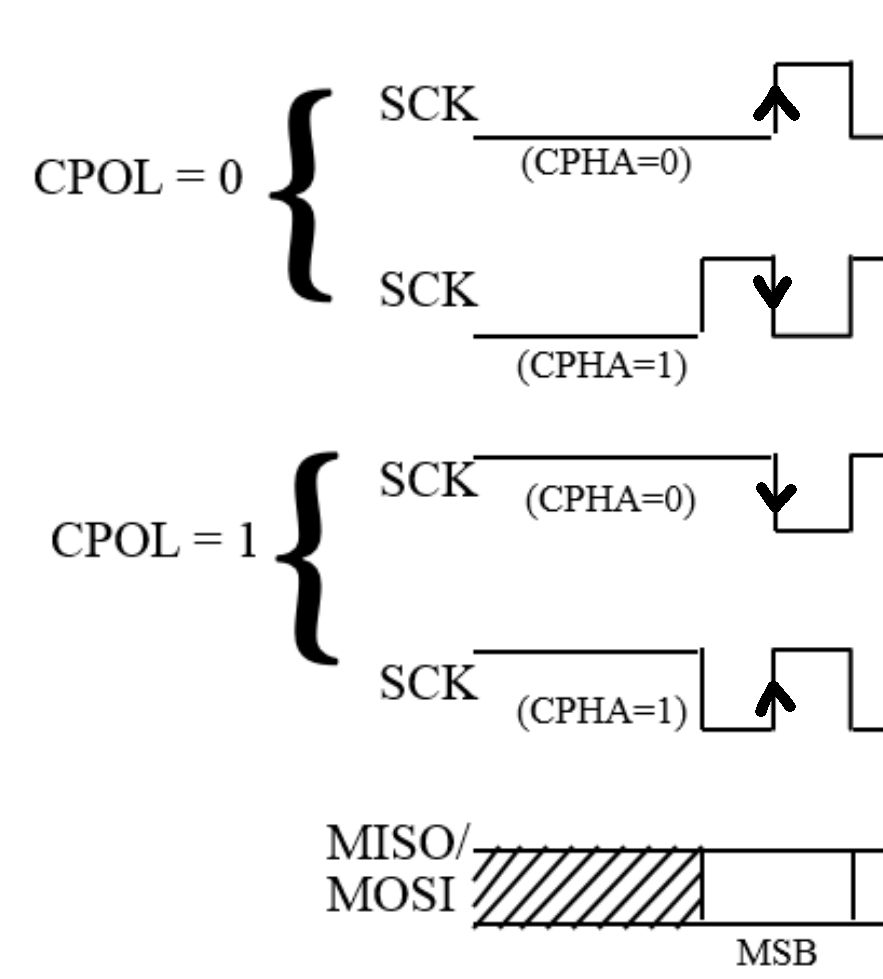
\includegraphics[width=.5\columnwidth]{"Images/SPI_Clock_modes.png"}
\end{center}

SPI can be setup in form of a Point-to-Point, Star or Ring topology.
There are implementations with multiple parallel datalines between master and slave (Dual-, Quad- Octal-SPI).


\subsection{I2C \refskript{9.4.2}}
See \refskript{Figure 9.25 and 9.26} for the message structure.
Max addresses: \formula{$2^{\text{\#-addr-bits}} - 16$} (Two 8-bit blocks are reserved).
For clock arbitration, see \refskript{Fig. 9.29}.

\begin{lstlisting}[language=C]
i2cError_t hal_i2c_dataRead(uint8_t slaveAddress, uint8_t* pData, uint8_t rxLen) {
	i2cError_t i2cError = I2C_NO_ERR;
	UCB1IFG = 0x0000;  // clear old flags
	
	// Set the address of the slave with which the master will communicate.
	UCB1I2CSA = slaveAddress;
	
	UCB1CTLW0 &= ~0x0010;  // receive mode
	UCB1CTLW0 |= 0x0002;   // generate start condition (start)
	while (UCB1CTLW0 & 0x0002);  // wait until start condition sent
	
	if ((UCB1IFG & 0x0020) == 0x00)  // check if no error occured
	{
		for (; rxLen > 1; rxLen--) {
			while (!(UCB1IFG & 0x0001)); // wait until receive is complete (RXIFG)
			*pData = UCB1RXBUF;  // get single byte data
			pData++;
		}
	} else {
		i2cError = I2C_ADDR_ACK_ERR;  // nack received --> no valid slave address
	}
	
	UCB1CTLW0 |= 0x0004;  // send as next the stop condition
	while (!(UCB1IFG & 0x0001)); // wait until receive is complete
	*pData = UCB1RXBUF;  // get last single byte data
	while (UCB1CTLW0 & 0x0004);  // wait until stop has complete sent
	return i2cError;
}
\end{lstlisting}

	\subsection{USB (Universal Serial Bus) \refskript{9.3.9}}
\subsubsection{Electrical characteristics}
\begin{itemize}
	\itemsep-.5em 
	\item Signals are NRZI (non return to zero inverted) encoded
	\item Bit stuffing is used for clock synchronization
\end{itemize}
\begin{center}
	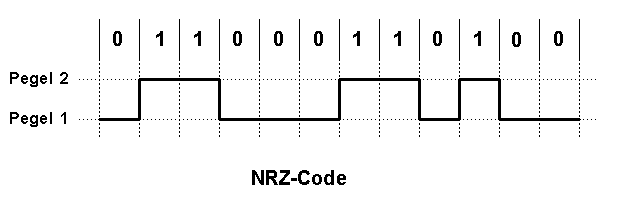
\includegraphics[width=.6\columnwidth]{"Images/NRZ_code.png"}
	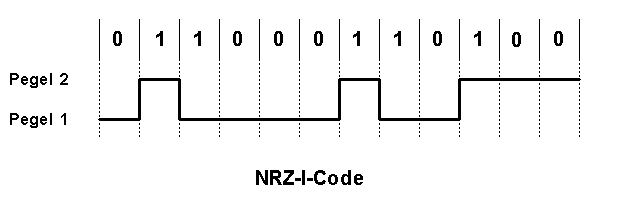
\includegraphics[width=.6\columnwidth]{"Images/NRZI_code.png"}
	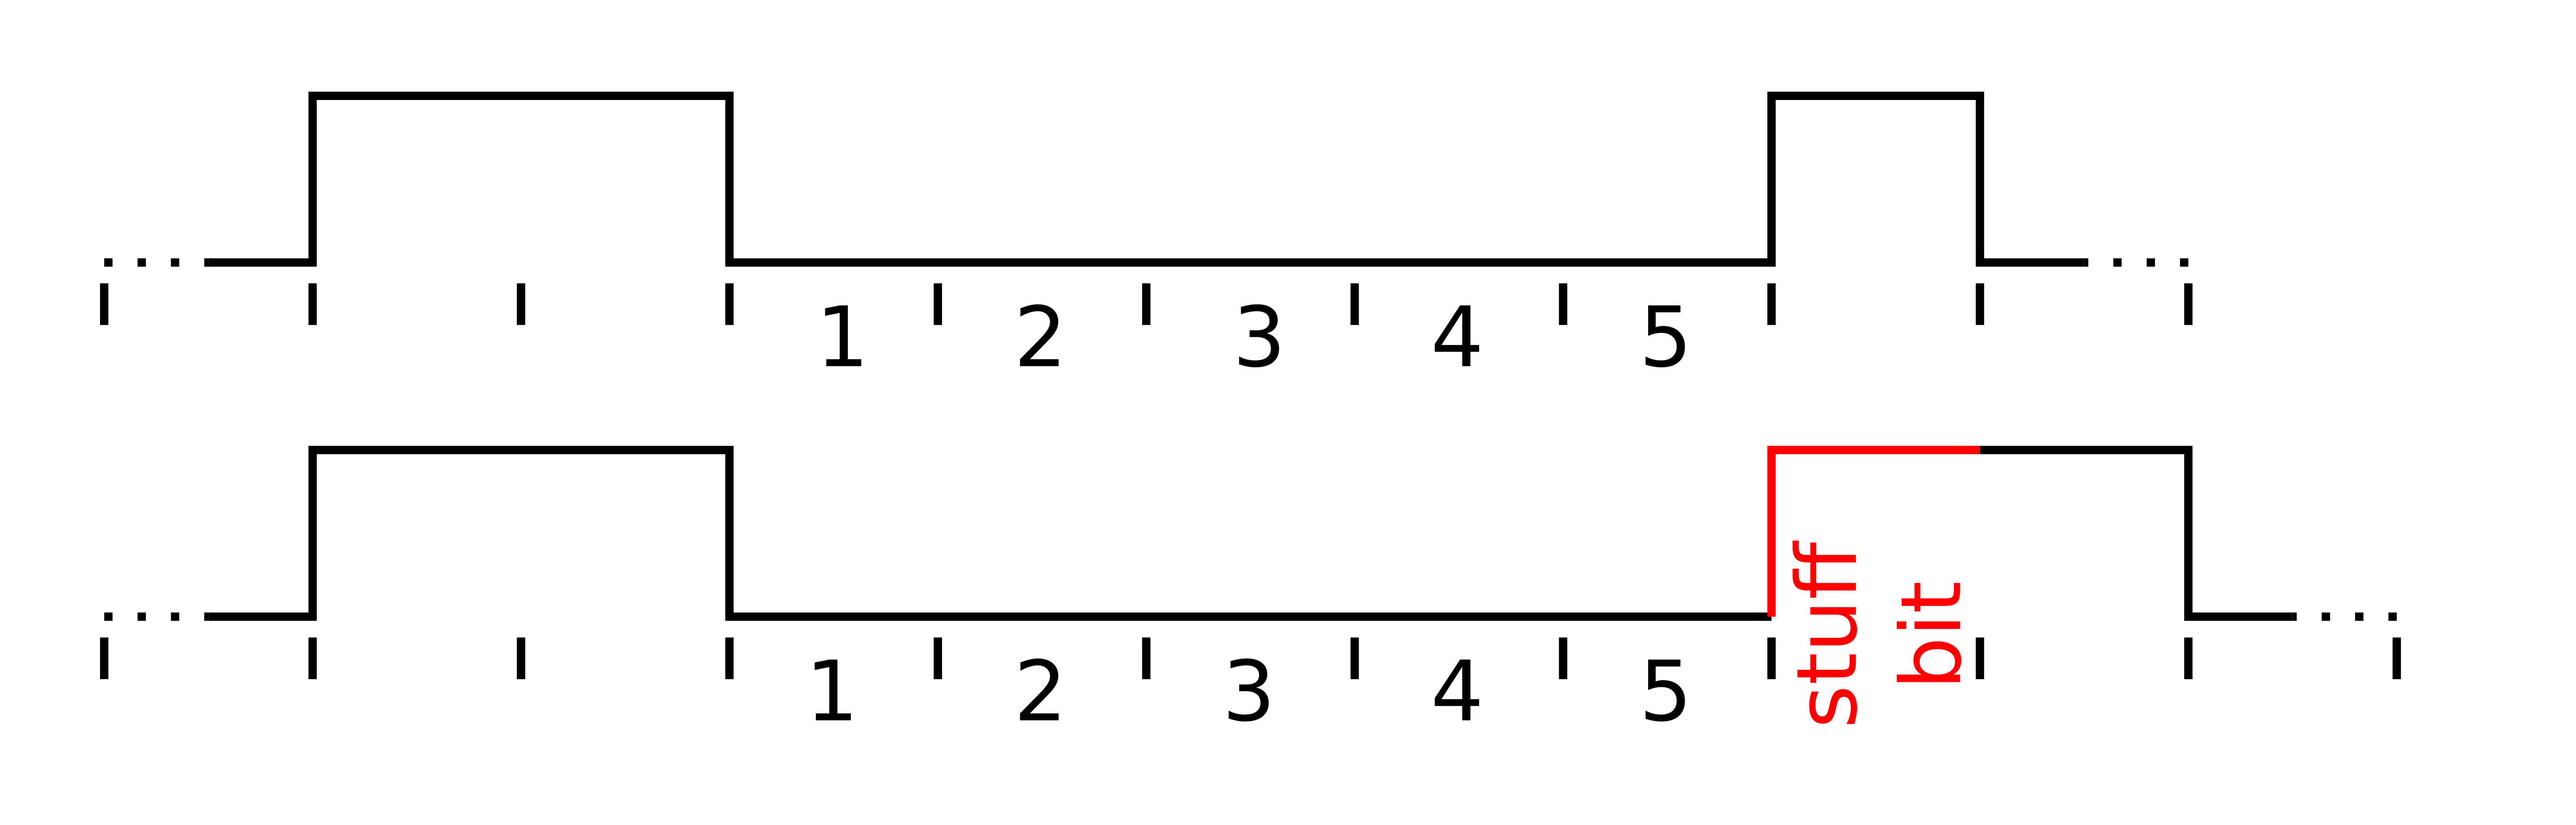
\includegraphics[width=.8\columnwidth]{"Images/BitStuffing.png"}
\end{center}

Each device can have up to total 32 \textbf{endpoints} (16 IN and 16 OUT).
There are different \textbf{packet types}, Token-, Data-, Handshake- and Start of Frame (SOF)- packets which are divided further into \textbf{packet fields} respectively.

There are four Transfer Types / Endpoint Types:
\begin{itemize}
	\itemsep-.5em
	\item Control: Always use of Endpoint 0 (IN \& OUT)
	\item Interrupt: Guaranteed quick responses
	\item Isochronous: Guaranteed data rate, possible data loss
	\item Bulk: Large data transfers using remaining bandwidth
\end{itemize}

USB OTG (On-The-Go) allows to directly connect two OTG capable devices because it can assume the host or the device role.


	\section{The Analog Signal Chain \refskript{10}}
\subsection{OpAmp \refskript{10.4}}
\subsection{Sampling and Quantization \refskript{10.7}}
\formula{$f_s \geq 2 \cdot f_H = f_n$}\\
\unitText{$f_s$}{Sampling Frequency}{Hz}\\
\unitText{$f_s$}{Highest Frequency}{Hz}

\subsubsection{Aliasing \refskript{10.7.2}}
\formula{$k \cdot f_s \pm f$}

Can be solved using a low-pass or band-pass filter.

\subsection{Quantization}
\formula{$\text{Quantization error} = \text{actual value} - \text{quantization level}$}\\
Full scale range: \formula{$V_{FS} = V_{max} - V_{min}$}\\
Resolution, precision: \formula{$\Delta = \dfrac{V_{max} - V_{min}}{2^n} = \dfrac{V_{FS}}{2^n} = \text{LSB resolution}$}\\

\subsection{Digital-to-Analog Converters \refskript{10.8}}
\subsection{Analog-to-Digital Converters \refskript{10.9}}
\begin{lstlisting}[language=C]
uint16_t hal_adc_sampleAndGet(adcChannel_t channel) {
	uint16_t result = 0x0000;
	
	// Disable ADC conversation (ENC-Bit)
	ADC12CTL0 &= ~0x0002;
	// reset conversion start address (bit4..0)
	ADC12CTL3 &= ~0x001F;
	// setup conversion start address (bit4..0)
	ADC12CTL3 |= (uint16_t)channel;
	// start sample and enable conversion
	ADC12CTL0 |= 0x0003;
	// wait while ADC-Unit is busy
	while (ADC12CTL1 & 0x0001);
	// read out result of memory0
	result = ADC12MEM0;  
	return result;
}
\end{lstlisting}
\end{document}


